% introduction and motivation slides


\begin{frame} %-----------------------------%
\frametitle{Motivation - Small Satellites} % small satellites
	\begin{itemize}
		\item Spacecraft design/launch and development are costly endeavors
			\begin{itemize}
				\item Long development timelines with extensive component testing
				\item Prohibitive launch costs and manifest scheduling
			\end{itemize}
			\pause
		\begin{table}
        \begin{tabular}{l | c | c }
        	Vehicle & LEO Capacity (\si{\kilogram}) & LEO Cost per \si{\kilogram} \\
        	\hline \hline
        	Space Shuttle & \num{28803} & \$ \num{10416}  \\ 
        	Atlas 2A & \num{8618} & \$ \num{11314} \\
        	Falcon 9 & \num{13150} & \$ \num{4654} \\
        	Falcon 9 Heavy & \num{53000} & \$ \num{1698}
        \end{tabular}
        \end{table}
		\item Small spacecraft enable cost effective and rapid development
	
			\begin{itemize}
				\item Reduced size/mass allows for `piggyback' on larger vehicles
				\item Cheaper designs allow for mass production/standardization 
			\end{itemize}

	\end{itemize}
\end{frame}   %-----------------------------%

\begin{frame} %-----------------------------%
\frametitle{Motivation - Low Thrust Transfers} % electric propulsion
\begin{itemize}
	\item Low-thrust orbital transfers
	\begin{itemize}
		\item Electric propulsion has increased in popularity

 		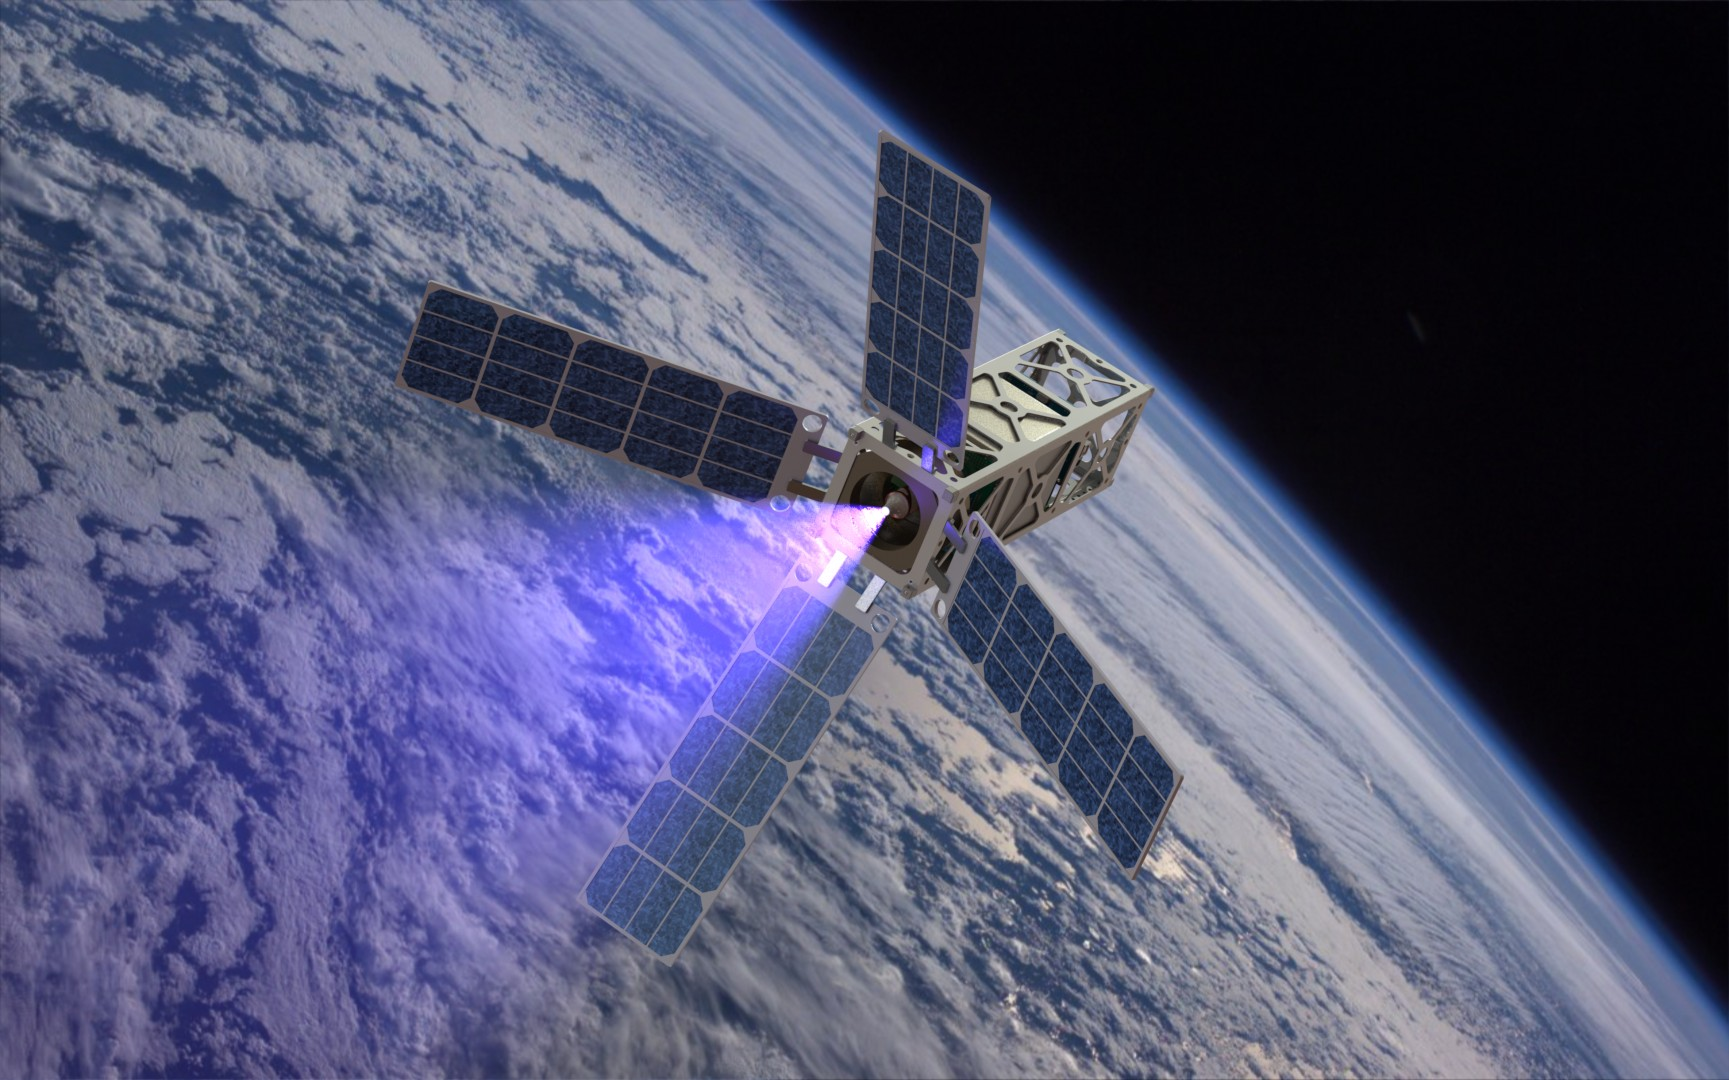
\includegraphics[height=0.3\textheight]{patriot_plume}
		\hfill
 		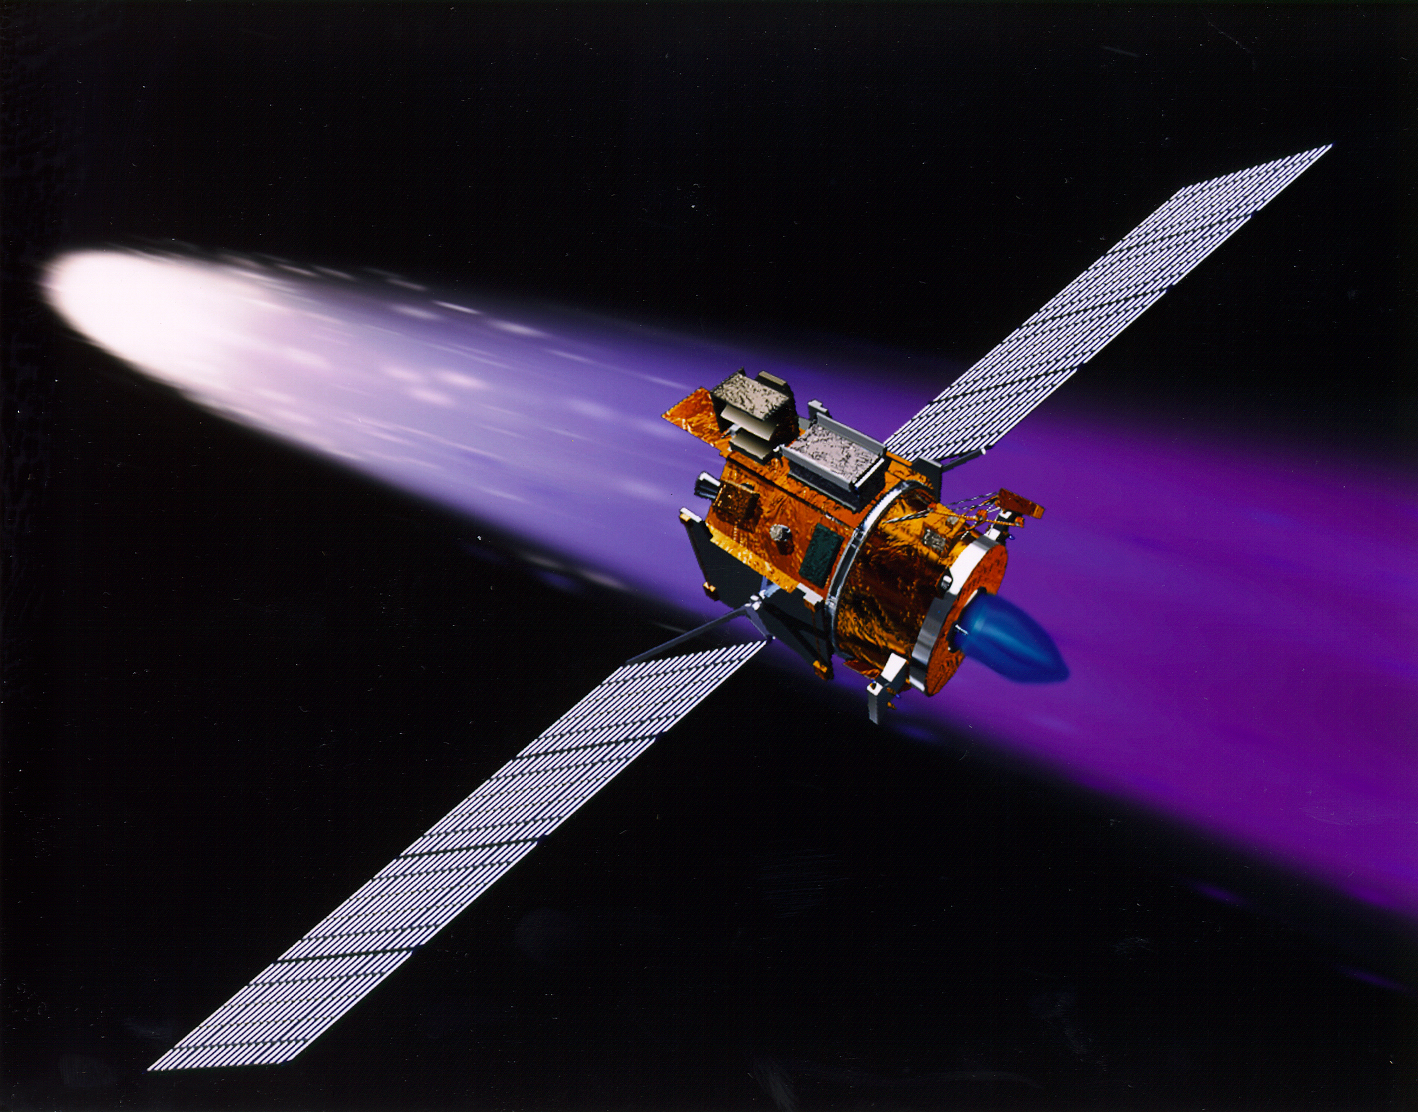
\includegraphics[height=0.3\textheight]{deepspace1}
 
		\item Offers much higher specific impulse than chemical engines 
		
		\item Requires much longer operating periods for maneuvers 
		\item Small satellites with electric propulsion allows for new mission types
			\begin{itemize}
				\item Formation flight (distributed aperture sensing)
				\item On-orbit servicing
				\item Interplanetary swarms
			\end{itemize}
	\end{itemize}
\end{itemize}
\end{frame}   %-----------------------------%